\chapter{Evaluation of Existing Applications}
\label{chp:3:EvalExisAppl}
After building a foundation by giving out an overview about the related work on personalized mass email communication, this section will evaluate existing applications available in the market. 

\section{Application Categories and Their Relation with the Thesis}
\label{sec:3.1:SystCate}

There are three different application categories related with this study that focuses on email communication either directly or indirectly. The following section will give a brief description of those categories, and their relation to this study:

\subsection{Customer Relationship Management (CRM)}
\label{subsec:3.1.1:Cust}
A \ac{CRM} application helps manage customer relationships effectively, a topic studied both by the academia and industry in the recent years. Such applications play an important role in the marketing field, where organizations use a more customer oriented approach instead of a product or brand-oriented marketing strategies. Therefore, each customer's economic value is different to the company, and the organizations' customer relation strategies require adapting their customer offerings and communication strategy personalized, according to individual customers \citep{Reinartz2004}. 
\vspace{1cm}

One of the reasons why this study considers on evaluating \ac{CRM} applications is because of the communication aspect of a company with their clients. Another reason is that as mentioned on section 2.3, the adequate amount of personalization in emails is crucial on the response rates, and people's increased daily interactions with the digital world makes true and authentic personalization rarer. Achieving such level of personalization requires getting to know each recipient very well by considering not only the recent conversations, but also earlier conversations. All the information that might be extracted from those conversations helps build a relationship with the respondents. Since a \ac{CRM} application aims to keep track of each customer's history regarding a product or a brand, such data storage could be leveraged to add an adequate amount of personalized information to email conversations. 

\subsection{Help Desk}
\label{subsec:3.1.2:HelpDeskSoft}
Another type of application that focuses on a company and its relationship with their clients is a help desk application. Its main purpose is to provide information and support related to a company's products and services offered to their customers. As a part of a knowledge acquisition, help desks support both sides of the communication in a way that customers or end users find the knowledge they need and the people who provide help by making the knowledge available and reusable \citep{Halverson2004}.
\vspace{1cm}

Reusing existing knowledge requires structuring of the captured knowledge. This is where it makes its connection to this study. A help desk application provides a workflow for both parties on developing an exchange of communication wherein a person who needs assistance describes his/her problem, while people who would provide help will then identify the solution to the problem by looking for similar earlier cases or by asking additional questions to clarify the initial problem. This also requires cooperation from assistants while providing help to a problem, at which one person might have a previous experience that can help guide the other assistants. As a result, a help desk application is similar to a mass email communication wherein a researcher initiates with an open-ended questionnaire, then extracts information from the coming replies, and organizes them according to the answers that he or she seeks for. In addition, respondents might also come up with additional questions to clarify things, where existing answers can easily be reused. Having such email conversations with large groups requires great effort from a researcher, so he might end up assigning tasks to distribute the efforts to other researchers in order to effectively deal with the demands of the large size of the group.


\subsection{Email Marketing}
\label{subsec:3.1.3:EmaiMarkt}
Organizations and marketers use email on marketing for several reasons. Some of those purposes are for brand and customer loyalty building, acquiring or converting customers, advertising the brand or the product, solicit sales or donation, communicating for promotional offers and even educational purposes. At the end, these approaches can be grouped under the following categories \citep{Eley2009}:

\begin{compactitem}
	\item \textbf{Educational Communication:} An educational message is given in the form of a newsletter, avoiding sale push, but it might still include some content encouraging recipients indirectly. For example, a free monthly newsletter which contains tips about digital photography, and photography accessories used in the tips might be linked to an online shopping website. 
	\item \textbf{News and Updates:} Used to notify the customers about important updates or changes to a business. For an instance, the release of a new product, changes on contact details or major changes on a company's website information.
	\item \textbf{Direct Sales Messages:} Emails sent out by others consists of marketing ads, and clear messages on offers.
	\item \textbf{Housekeeping:} Emails such as subscriptions for confirmation messages or welcome emails. These messages are often to be system generated or automated messages. However, they can be used to promote messages as well as offering a discount code along with the registration of the confirmation email.
\end{compactitem}

Since these categories consist of a communication with a large group of people, this study also evaluates existing tools available in the market for email marketing, including their technical aspects.

\section{Methodology}
\label{sec:3.2:Meth}

The analysis examined two products from each of the categories --- \ac{CRM}, Help Desk, and Email Marketing. The selection of the products depends on several product comparison websites, including Toptenreviews.com\footnote{http://\{email-marketing-software-review, crm-software-review\}.toptenreviews.com/ }, Softwareshortlist.com\footnote{http://www.softwareshortlist.com/crm/solutions/}, as well as the suggestions of Stanford HCI group members\footnote{http://hci.stanford.edu/people/}. In addition to those websites and suggestions, their demo or trial version availability was also considered, since some of the products actually require a certain fee before using them. After the products were shortlisted, the last filtering was done by getting their web traffic rankings from Compete.com\footnote{https://www.compete.com/}, Alexa\footnote{http://www.alexa.com/}, and Google Trends\footnote{http://www.google.com/trends/}. Finally, the trial accounts of those applications were created, and a scenario was simulated to get the full insight from them. 

\section{Results}
\label{sec:3.3:Resul}
Evaluation of the products will be performed according to their respective categories. A brief description of the product will be presented, as a part of its evaluation. This description will mainly focus on the product's features, which is related to support email communication, as explained in section~\ref{sec:3.1:SystCate}. Afterwards, each category will then be a conclusion, including a comparison matrix of the selected products.

\subsection{CRM Applications}
\label{subsec:3.3.1:CRMAppl}

SugarCRM and Highrise are the two \ac{CRM} applications that were analyzed in this study. Table~\ref{tab:comp_matr_crm} shows a summary of their features, and the following paragraphs will give a more in-depth exploration for these products.

\clearpage

\begin{table}[H]
\begin{center}
	%\renewcommand{\arraystretch}{2}
	%\tiny
	%\setlength{\tabcolsep}{5pt}
	\caption[Comparison Matrix for CRM Applications]{Comparison Matrix for CRM Applications} \label{tab:comp_matr_crm}
    \begin{tabular}{ | p{3cm} | p{5cm} | p{5cm} | }
	\hline
	& \textbf{SugarCRM} & \textbf{Highrise} \\ \hline
	\textbf{Versions} & On-premise and SaaS & SaaS \\ \hline
	\textbf{Pricing} & \$35 -- \$100 user/month, and a free community edition & \$24 -- \$99/month, and a free plan with limitations \\ \hline
	\textbf{Task Management} & Calendar based, no additional view & Individual module \\ \hline
	\textbf{Syncronization} & Plugins are available for Outlook, Lotus Notes & Requires additional module installation \\ \hline
	\textbf{Email Client} & Built-in, allows email marketing with variable insertions & No \\ \hline
	\textbf{Contact Importing} & Via forwarding emails or plugins for Outlook, Lotus Notes & Outlook, Excel, vCard, or via forwarding emails \\ \hline
	\textbf{Mobile Support} & Yes & No \\ \hline
	\textbf{Analytics} & Marketing Analytics, sales forecasting and trends & No \\ \hline
    \end{tabular}
\end{center}
\end{table}

\paragraph{SugarCRM}
SugerCRM comes in three different deployment versions: On-premise, \ac{SaaS} and the free community edition. It has a clean \ac{UI} with a single navigation menu. Its calendar view can be synchronized with Outlook's calendar or any other platform's, which supports iCalendar\footnote{iCalendar is the calendar data exchange standard (RFC 5545) having file extension of .ics, and it allows sending meeting requests or tasks via email.}. It has a built-in email management feature, as well as integrations with several platforms like Outlook and Gmail, or an \ac{IMAP} based email server. Users can archive emails in the SugarCRM application by adding a unique email address into the TO, \ac{CC} or \ac{BCC} fields. This address can also be used to link an email recipients' information, including email attachments with SugarCRM by simply forwarding the emails. Therefore, it removes the additional effort on manually importing them into the SugarCRM application and reduces dependency on a platform. The SugarCRM also comes with a built-in email client. Even though its inbox view can only provide basic functions, its email creation view goes a little further in supporting email marketing by providing dynamic variables that can be embedded into an email's content that can be replaced with actual values available in the SugarCRM application. For example, a variable for "first name" will be replaced by a contact's actual first name while email is being sent (See figure~\ref{fig:SugarCRM-Create_Email}). 
\vspace{1cm}

\begin{figure}[htbp]
	\centering
	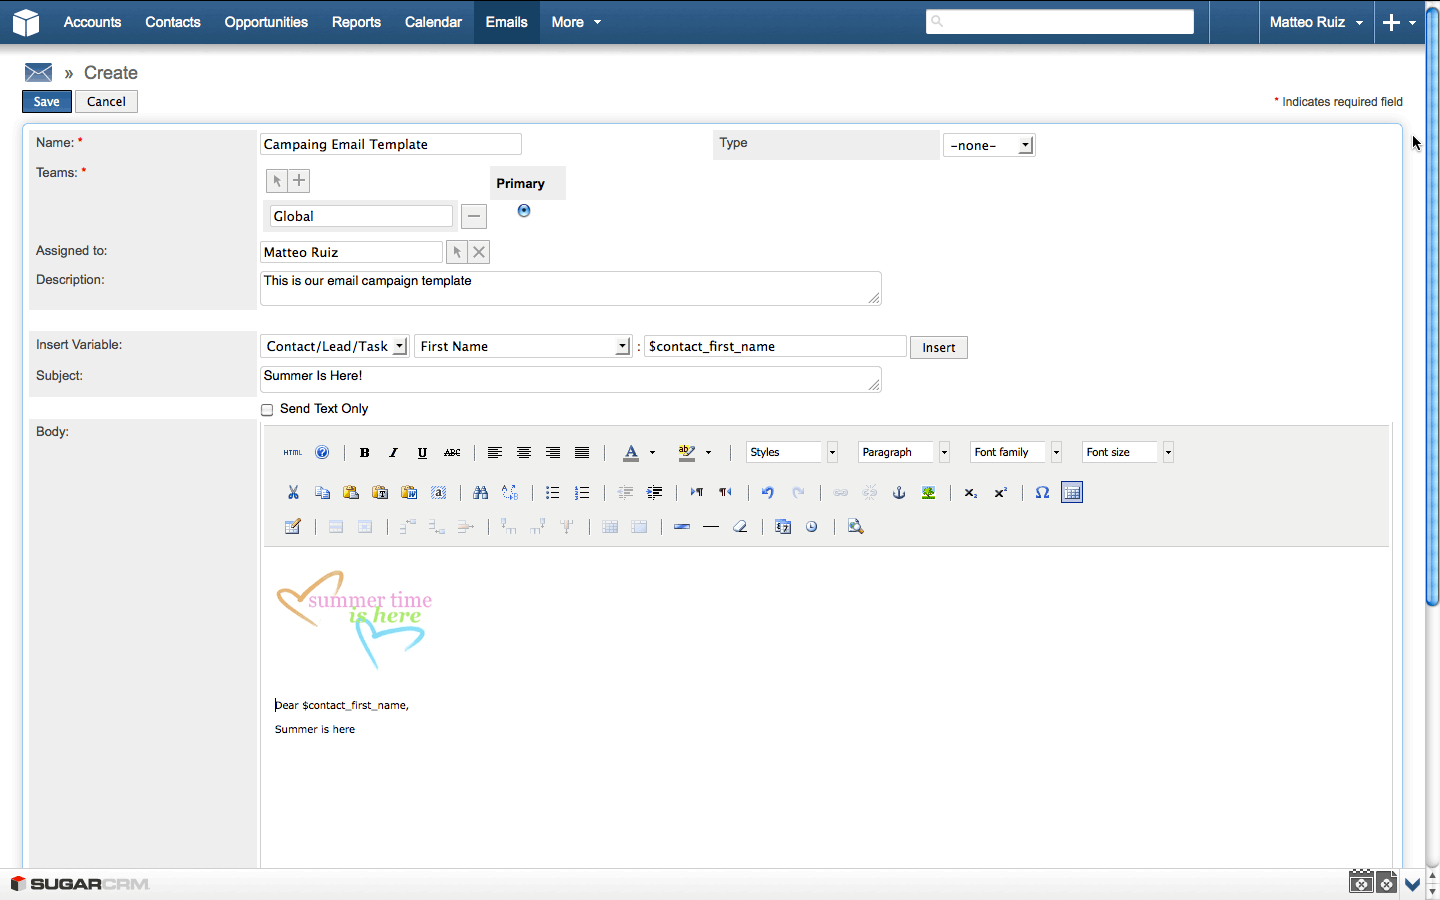
\includegraphics[width=1.00\textwidth]{imgs/SugarCRM-Create_Email.png}
	\caption[SugarCRM Email Composer with Embeded Variables]{SugarCRM Email Composer with Embeded Variables \citep{SugarCRMInc.2013}}
	\label{fig:SugarCRM-Create_Email}
\end{figure}

Initiated email marketing can be monitored to track response rates, generated leads, and unsubscribed contacts. A marketing target lists can also be imported from third-party lists. The SugarCRM also let users save an email as a \ac{HTML} template, allowing the user to use it again within an email composer. Finally, it offers a mobile version, allowing users to easily access most of the application's features using their smartphones and tablet devices \citep{SugarCRMInc.2013}.

\paragraph{Highrise}
Another \ac{SaaS} application available on the market is Highrise\footnote{http://highrisehq.com/}. It offers several purchasing plans, with a 30-day free trial period. It has a simple \ac{UI} like the SugarCRM, but it also has quick access buttons for adding a task or a contact. The task management feature on the Highrise application makes it different from the SugarCRM, since unlike the latter, instead of a calendar view, it offers a task view, which can be synchronized with iCalendar as well. In addition, users can create tasks from emails by using one of the unique email addresses for several time slots provided by Highrise, and adding them into \ac{BCC}, \ac{CC}, or simply by forwarding an existing email, creating a task in Highrise. Contact information can be imported from Outlook or by uploading a vCard\footnote{vCard is a file format standard for exchanging business contact information.} file. It provides all the basic contact information fields, including social accounts; however, it does not offer custom field creation on those profiles. An email, including its attachments, can also be linked to a contact profile just by simply forwarding it to the provided unique email address. If a user does not exist in the Highrise contact database when an email from him or her was forwarded to link it, a contact profile is created using any available information in that email. Adding tags to contact profiles also makes it easier to organize contacts and browsing within them. However, the Highrise application does not offer an email composer to do an email marketing, as seen in the SugarCRM application. Therefore, users will have to depend on a different third-party application to do simple email campaigns. The provided activity view helps users on keeping track of their own or other users' recent actions within the Highrise application. Lastly, it offers options on customizing the look and feel of the application with the use of the system provided color schemes, depending on the user's preference \citep{37signals2013}.

\subsection{Help Desk Applications}
\label{subsec:3.3.2:HelpDeskAppl}

The two help desk applications reviewed in this study are Zendesk and Kayako. Table~\ref{tab:comp_matr_help} provides a comparison matrix of their features, and the details are described in the following paragraphs.

\clearpage

\begin{table}[H]
\begin{center}
	%\renewcommand{\arraystretch}{2}
	%\tiny
	%\setlength{\tabcolsep}{5pt}
	\caption[Comparison Matrix for Help Desk Applications]{Comparison Matrix for Help Desk Applications} \label{tab:comp_matr_help}
    \begin{tabular}{ | p{3cm} | p{5cm} | p{5cm} | }
	\hline
	& \textbf{Zendesk} & \textbf{Kayako} \\ \hline
	\textbf{Versions} & SaaS & Software and SaaS \\ \hline
	\textbf{Pricing} & \$24 -- \$119 agent/month, with a limited free trial version & \$29 -- \$49 user/month, with a limited free trial version \\ \hline
	\textbf{Channels} & Website, email, phone, and social platforms & Website, email, and only the Fusion version supports phone \\ \hline
	\textbf{Macros} & Yes, basic & Yes, advanced \\ \hline
	\textbf{Ticket Management} & Groups and tags & Types, statuses, priorities, and tags \\ \hline
	\textbf{Mobile Support} & Yes & No \\ \hline
	\textbf{Analytics} & Yes & Yes \\ \hline
    \end{tabular}
\end{center}
\end{table}

\paragraph{Zendesk}
Cloud-based customer service software Zendesk \footnote{http://www.zendesk.com} provides a nice and clean \ac{UI}. Zendesk has more than 30,000 businesses from a wide variety of industries. Zendesk offers one-on-one support through different communication channels including a company's website, email, phone, and social media platforms like Facebook and Twitter. Hence, support requests coming from those platforms can be turned in to a support ticket, and those support tickets can be grouped under categories, and further classification can be done via tags for each ticket. This feature also helps in finding related archived resolved tickets, so they can be reused for new tickets. Thanks to the automated process coming with macros, a combination of actions can be done with a one-click like setting status, priority, type of a ticket, and assign it to another person with a predefined comment for the ticket. A ticket can be merged with another one, or copied to the forum to make it available to the public, which helps creating a reliable knowledge base. Customer ticket histories and basic personal information are kept in the system. However, it does not allow adding additional fields on the customers' profiles. In addition to the desktop version, Zendesk has a mobile version for smartphones and tablet devices. Therefore, the support team does not have to depend on the desktop platform, as long as they have it on their mobile devices as well. Lastly, the provided analytics view by reports gives an overview of customer satisfaction, and performance of the support team \citep{Zendesk2013,Zendesk2013a}.

\paragraph{Kayako}
Kayako's\footnote{http://www.kayako.com/} complete solution for customer support is named as Kayako Fusion. It comes as software and \ac{SaaS}. Kayako has more than 30,000 clients within the last ten years. Unlike Zendesk, using its \ac{UI} seemed to be a little more complicated than the latter, and does not have a social media integration, therefore support tickets are generated only over a company's website, or via email and phone. Tickets can have customized types, statuses, priorities, and tags. Similar to Zendesk, it also supports macros to assign tickets into a department, owner, type, priority, and provide canned responses for tickets with just a single click. Kayako also keeps basic information of customers, as long as they are registered in the system. Registered customers can also participate in building knowledge base in a forum-like environment by answering other customers' questions together with a support team. However, Kayako does not have a native app for smartphones and tablet devices like Zendesk. Finally, it has an analytic view to keep track of ticket reports, measuring customer satisfaction and support team's performance \citep{KayakoInc.2013,KayakoInc.2013a}.

\clearpage

\subsection{Email Marketing Applications}
\label{subsec:3.3.3:EmaiMarktAppl}

MailChimp and Constant Contact are the chosen email marketing applications to be reviewed in this study. Table~\ref{tab:comp_matr_emai} shows an overview of their features on a side-by-side comparison to. Supporting details are provided in the following paragraphs.

\begin{table}[H]
\begin{center}
	%\renewcommand{\arraystretch}{2}
	%\tiny
	%\setlength{\tabcolsep}{5pt}
	\caption[Comparison Matrix for Email Marketing Applications]{Comparison Matrix for Email Marketing Applications} \label{tab:comp_matr_emai}
    \begin{tabular}{ | p{3cm} | p{5cm} | p{5cm} | }
	\hline
	& \textbf{MailChimp} & \textbf{Constant Contact} \\ \hline
	\textbf{Versions} & SaaS & SaaS \\ \hline
	\textbf{Pricing} & \$10/month with max 500 subscribers -- \$240/month with max 50,000 subscribers. Pay as you go available & \$15/month with max 500 subscribers -- \$75/month with max 10,000 subscribers. \\ \hline
	\textbf{Template Editor} & Drag and drop including advanced photo editor & Drag and drop including basic photo editor \\ \hline
	\textbf{Recipients List} & Conditional filtering & Grouping \\ \hline
	\textbf{Variable Support} & Yes, advanced & No \\ \hline
	\textbf{Permissions} & Admin, manager, author, and viewer account types & None \\ \hline
	\textbf{Mobile Support} & Yes & No \\ \hline
	\textbf{Analytics} & Yes & Yes \\ \hline
    \end{tabular}
\end{center}
\end{table}

\paragraph{MailChimp}
MailChimp\footnote{http://mailchimp.com/} comes as \ac{SaaS}, and offers either a fixed monthly plan or a pay as you go plan. Along with its intuitive \ac{UI}, it offers a drag-and-drop function on the email content creation. It supports email marketing processes ranging from designing the sign-up form so that users can add their desired fields and apply brandings on it to applying personalization on emails using dynamic variables. The recipients' list can also be filtered out according to several conditions like their campaign name, location or ratings, as assigned by the user. There are different user account types with different levels of privileges in accessing MailChimp. A person who has an "Admin" account is the only one capable of granting permissions to other users, as well as determining one's access limitations on using MailChimp. This allows an efficient way for the distribution of mail marketing tasks. For an instance, while the assigned manager manages the recipients list, the author team can focus on the emails' content and design \citep{TheRocketScienceGroupLLC2013}. To design an email content, users can either decide on picking an available template from a collection provided by the MailChimp application or to create their own \ac{HTML} templates with its drag-and-drop editor (See figure~\ref{fig:MailChimp-DragAndDropEditor}).
\vspace{1cm}

\begin{figure}[H]
	\centering
	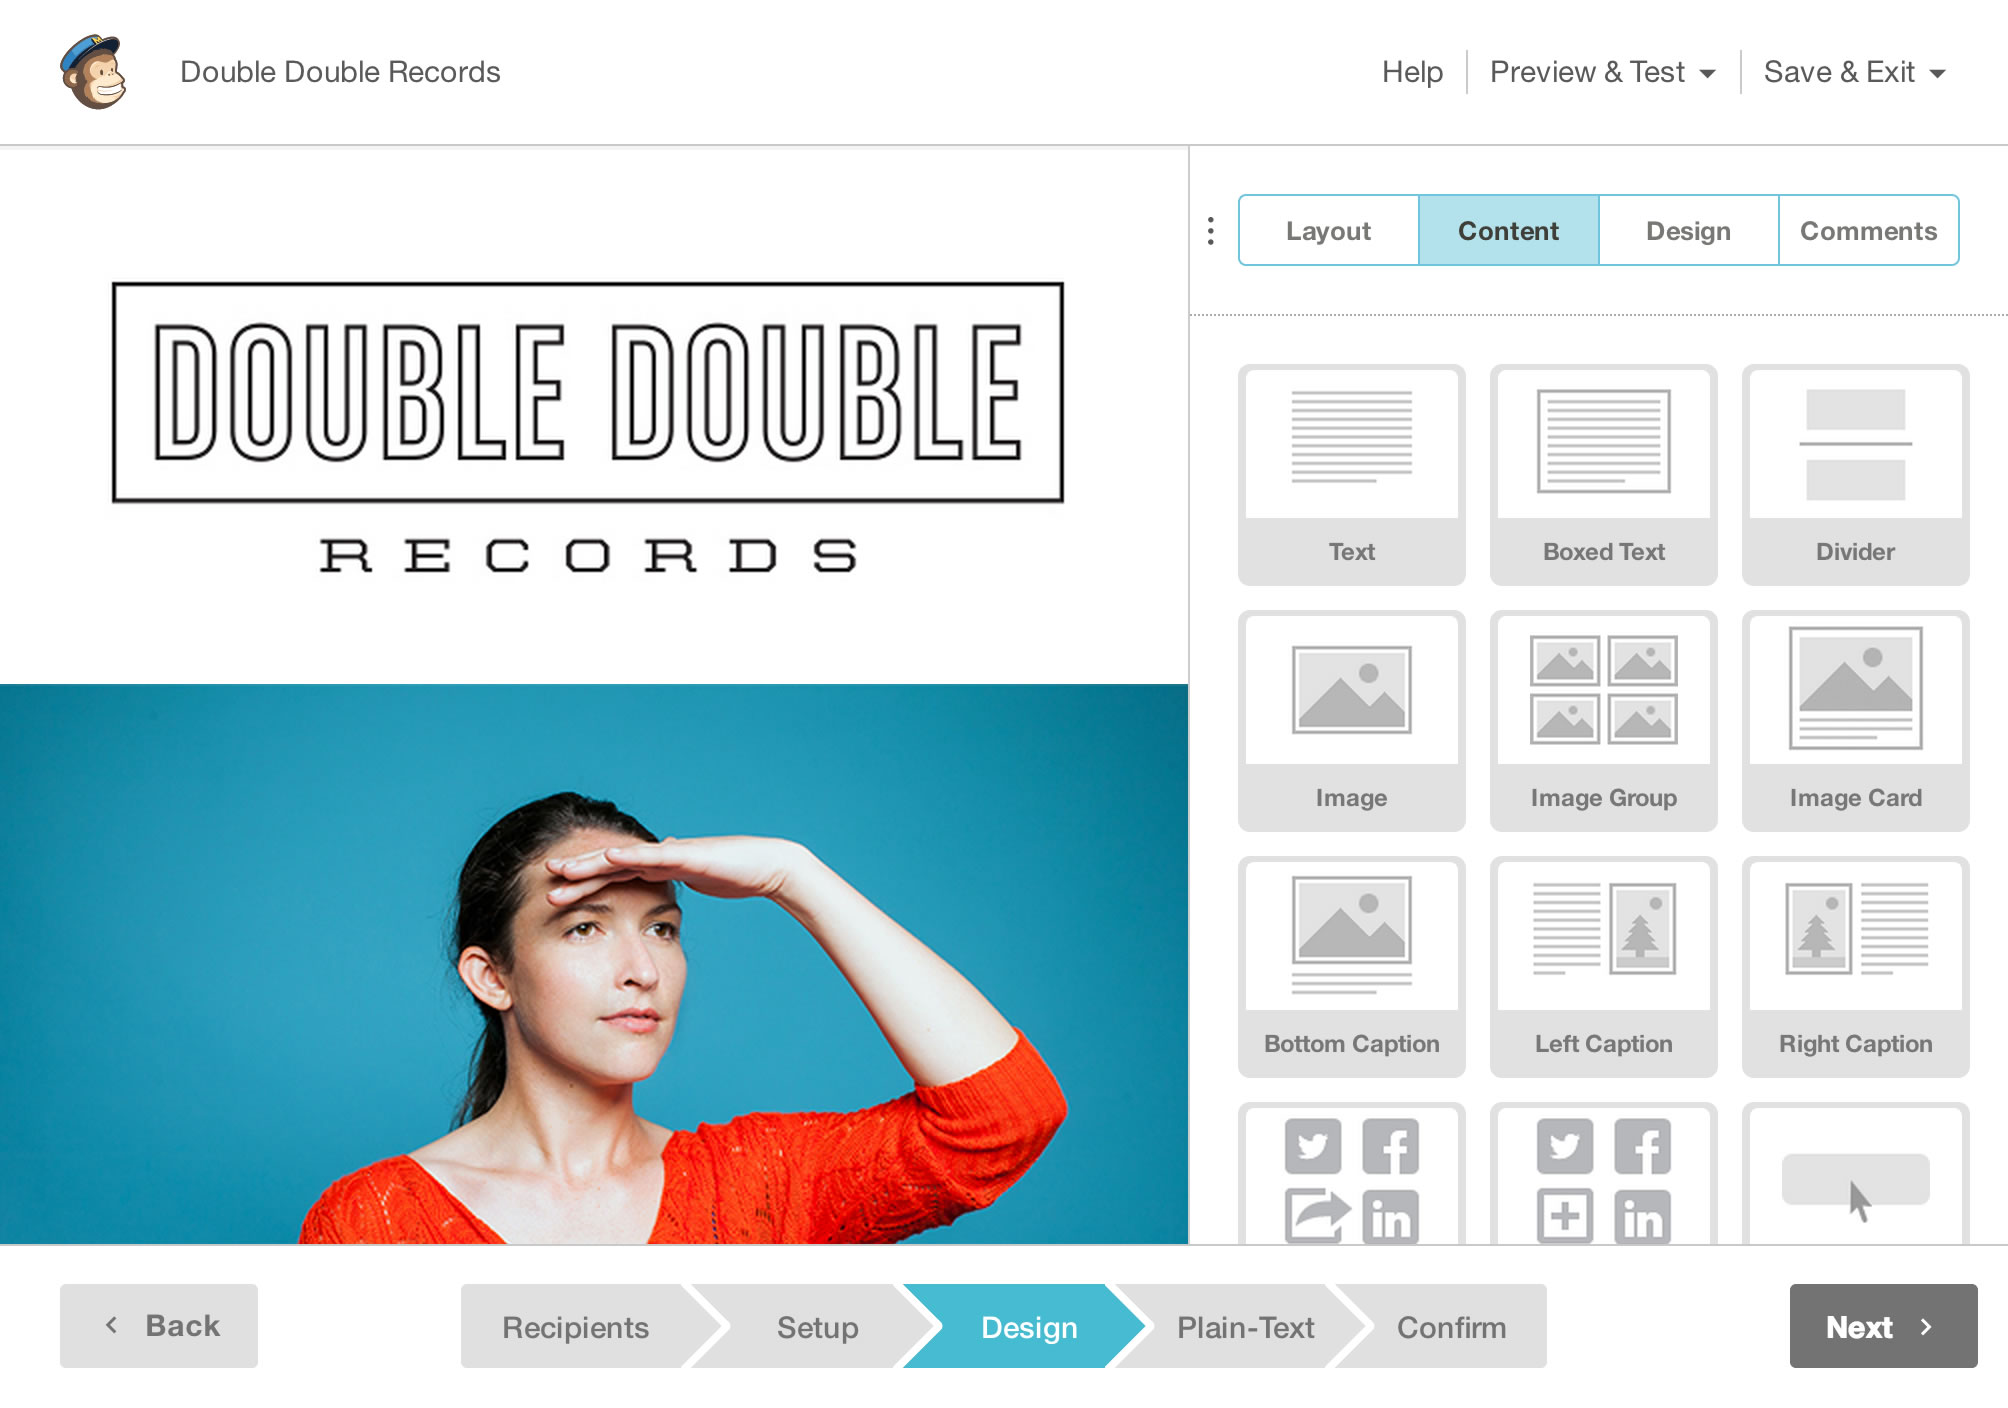
\includegraphics[width=1.00\textwidth]{imgs/MailChimp-DragAndDropEditor.jpg}
	\caption[MailChimp Drag-and-Drop Content Editor]{MailChimp Drag-and-Drop Content Editor \citep{TheRocketScienceGroupLLC2013a}}
	\label{fig:MailChimp-DragAndDropEditor}
\end{figure}

The template editor has a photo editing feature, and authors can add comments to give a feedback on the content and design of the templates. Created templates can be previewed as if they are viewed on either a software email client, an web-based email client, or even on a mobile web browser \citep{TheRocketScienceGroupLLC2013a}. Similar to the SugarCRM application, MailChimp allows you to use dynamic variables --- merge tags --- in the email content. Therefore, sending out emails can be personalized with recipient-specific information. However, it provides more types of dynamic variables than SugarCRM, and it is possible to add a conditional logic to them. For example, in listing~\ref{lst:MailChimCondMergTags}, a custom discount message will be shown in the email depending on what state in the US the recipient is from.
\vspace{1cm}

\lstset {
 basicstyle=\footnotesize,
 frame=shadowbox,
 rulesepcolor=\color{black},
 showspaces=false,showtabs=false,tabsize=4,
 numberstyle=\tiny,
 captionpos=b,
 xleftmargin=0.7cm, xrightmargin=0.5cm,
 lineskip=-0.1em,
 abovecaptionskip=1\baselineskip
}

\begin{lstlisting}[language=XML, caption={[MailChimp's Conditional Merge Tags]MailChimp's Conditional Merge Tags \citep{TheRocketScienceGroupLLC2013b}}, label={lst:MailChimCondMergTags}]
	*|IF:STATE=CA|*
		Save 20% on surf boards!
	*|END:IF|* 
	*|IF:STATE=GA|*
		Save 20% on Mountain Bikes!
	*|END:IF|* 
	*|IF:STATE=FL|*
		Save 40% on water skis!
	*|END:IF|* 
	*|IF:STATE=CO|*
		Save 50% on ski gear
	*|END:IF|*
\end{lstlisting}

MailChimp also offers an auto-response feature, based on a triggering event. These events can be a clickable link in the email, a specific date like birthday of a contact, or scheduled dates. Finally, an analytics dashboard is present, where users can track the amount of opened emails, or the click rates of the links in the emails \citep{TheRocketScienceGroupLLC2013c,TheRocketScienceGroupLLC2013d,TheRocketScienceGroupLLC2013e}.

\paragraph{Constant Contact}
Another email marketing \ac{SaaS} is the Constant Contact Email Marketing\footnote{http://www.constantcontact.com/email-marketing}, whose purchase plan depends on the number of contacts you have, but a free 60-day trial period is available upfront. It offers a drag-and-drop content creation on a clean \ac{UI} like MailChimp's. It offers quite a number of templates to choose from and customize. Users can embed sign-up forms into their websites or Facebook accounts. The recipients list can also be imported from different sources like Microsoft Excel, Outlook, and Gmail. In addition, recipients can be grouped into sub-lists, which can also be merged into each other easily. An option of removing duplicate contacts from the lists or delete recipients who unsubscribed from the list is also available. Users can track how many opens, clicks, forwards, and social media platform shares are done for their email campaign. On the other hand, it does not offer any sophisticated email variables to be replaced by an actual content from the application \citep{ConstantContactInc.2013,ConstantContactInc.2013a,ConstantContactInc.2011}. 

\clearpage

\section{Conclusion}
\label{sec:3.3:Conc}
In conclusion, the aforementioned applications in three different categories provide support for the email communication in several ways:

\begin{compactitem}
	\item Contact User profiles kept in the \ac{CRM} applications can help a researcher to get to know their respondents better and to identify basic attributes like their name, gender, address, and phone numbers. However, fields are non-customizable, and are limited to the fields provided by the application.
	\item Importing contact information from other popular software, e.g. Outlook, can ease the time on creating recipient lists for email communication. SugarCRM and Highrise supports importing an email into the system by just simply forwarding it to a specific email address, making a researcher's life easier. Providing such flexibility will reduce the dependency on a platform, therefore, as the researchers continue on using the email clients they are familiar with, they can easily switch to another platform whenever it is necessary.
	\item Both \ac{CRM} applications reviewed provides a module on creating tasks, which can be helpful on reminding researchers on the things they need to do, for their email campaign, depending on their priority level. It works like a task showing the next thing to do in an email campaign, as initiated by the researcher. For an instance, sending a reply to an email in which a respondent asked a question clarifying something about the initial campaign.
	\item Both \ac{CRM} applications provide support on the archiving of emails by simply forwarding them to a provided unique email address, and linking those emails to the users' profile. This can be very helpful on looking for important conversations with respondents on an earlier time, to provide content or opinion on how to initiate upcoming conversations with those people. However, forwarding an email is an additional step, which requires additional effort and time.
	\item Reusability of earlier emails is important, so you do not have to write them again. As we have seen, the SugarCRM application also allows saving emails as a template for future use. However, no filtering mechanism or a similar function is available, but by just remembering the given name of the template helps the users find the corresponding template to use.
	\item Not all the time a researcher would be the first one to initiate the communication via email. Sometimes, a number of emails might be sent to a researcher's email inbox for inquiries or whatnots. For example, students attending a course may ask questions or some clarifications regarding their homework. Given the scenario, similar or identical questions might be asked several times. A help desk application provides a ticketing system for customer related issues, which is also applicable to the above-mentioned scenario. Therefore, existing email replies can be reused for further recipients.
	\item Both help desk applications support tagging or grouping of incoming emails, which can be helpful in identifying conversations related to a specific situation where a researcher initiated more than one campaign. However, there was no available visual representation of the state of the communication of a support ticket, but just status labels like "resolved" or "assigned".
	\item Another feature of a help desk application is a support ticket that can be shared or assigned among the members of the support team, which helps decrease the time needed to answer those tickets. This can be also useful in a mass email communication to share the responsibility of replying or extracting information from incoming emails.
	\item The email marketing application MailChimp provides dynamic variables that let users add into their email content and its variable will be replaced with actual value. Such a feature can be helpful in a personalized mass email communication, where it is difficult and very time consuming on adding recipient specific personalized information into emails. However, there is no attached information on those variables showing users what part of the communication exchange they were extracted, and again they are separately created --- an additional view where users are away from the actual emails where they can extract information.
	\item MailChimp also provides different types of permissions to leverage in an email marketing task. For an instance, as the author creates the email content, a viewer can just follow the reports to see what the success rate of an initiated campaign is. Such functionality can also be helpful in mass email communication, where some users can extract the information from the emails so others can easily reply to them.
	\item Both of the email marketing and help desk applications provide analytic reports to keep track of the success of a campaign or a support team. This is a very useful function in a mass email communication, as well as to getting a quick overview of the current state of the communication.
\end{compactitem}

As mentioned above, there are many useful features that can be helpful to ease a mass email communication. However, there is no one specific application capable of doing all of the mentioned features, or doing them in a way to support their main purposes, which are \ac{CRM}, help desk, and email marketing.

\begin{comment}
As it is mentioned in~\ref{sec:2.3:PersEmai}, recipients intense daily interaction with digital devices make the true authentic personalization rare, and resulting low response rates. Therefore, it is important to have a platform where researchers can easily extract information, and leverage them again for the personalization of further email communication too.
\end{comment}

\vspace{1cm}

In the next section, an initial prototype will be introduced to support the workflow of a personalized mass email communication.

\begin{comment}
--> At the end, put the all the comparison tables together to the Appendix
--> These features are also helped us to add them into our app, decided by saying they all support so we can also support
--> HDesk provides reusibility of emails, CRM provides contact details to replace in email content
\end{comment}
